\chapter{Studio di vulnerabilità}
\label{cap5}

Il concetto di \textbf{vulnerabilità} in una rete complessa mira a \textit{quantificare} la sua \textit{sicurezza} e la sua \textit{stabilità} sotto gli effetti di un qualsiasi tipo di \textit{disfuzione} \cite{MattssonJenelius2015}.

Nelle PTN la vulnerabilità è legata alla \textit{sensibilità alle interruzioni}, in particolare una definizione consolidata e diffusa è la seguente: "\textit{La vulnerabilità in un sistema di trasporto è la suscettibilità ad incidenti che possono portare ad una considerevole riduzione della funzionalità della rete stessa}" \cite{Berdica2002}. 

\section{vulnerabilità in una PTN}
Per studiare la vulnerabilità, bisogna prima comprendere cosa si intende con \textit{attaccare} una rete. \\
Un \textbf{attacco} in una rete è la rimozione intenzionale di nodi o archi con l’obiettivo di ridurre la funzionalità o connettività del sistema \cite{vonFerber2012LondonParis}, può essere eseguito secondo due approcci:
\begin{itemize}
    \item \textbf{Statico} in questo approccio non si considerano gli effetti della rimozione di un nodo, ovvero si assume che, eliminando un nodo, il resto della rete sia comunque operativa;
    \item \textbf{A cascata} in questo approccio, più realistico, si considerano gli effetti della rimozione di un nodo, ovvero si rimuovono i nodi non seguendo l'ordine di rimozione stabilito inizialmente, ma ricalcoldando ogni volta la metrica di riferimento.
\end{itemize}

\subsection{Ordine di attacco}
Nell'analisi di vulnerabilità l'obiettivo è portare la rete allo stremo per studiarne il comportamento in situazioni di gravità crescente, quindi non si rimuove un solo nodo, ma una \textit{successione di nodi} secondo un determinato criterio. Il criterio prescelto discrimina l'attacco in due tipologie:
\begin{itemize}
    \item \textbf{Attacco mirato} si rimuovono progressivamente dei nodi selezionati per importanza, nel caso in studio si effettuerà un attacco mirato per \textit{grado} e uno per \textit{betweenness};
    \item \textbf{Attacco casuale} si rimuovono progressivamente e casualmente dei nodi.
\end{itemize}

\subsection{Criterio di integrità}
Una volta stabilito cosa si intende con \textit{attacco}, bisogna comprendere come \textit{quantificare} gli effetti dell'attacco, ovvero comprendere quanto la rete è \textbf{integra}. \\
Il \textbf{criterio di integrità} più utilizzato \cite{vonFerber2012LondonParis} passa per il concetto di \textbf{componente connessa}: gli effetti di un attacco si comprendono analizzando come varia, in termini di quantità di nodi, la più grande componente connessa della rete.

Si introduce quindi la \textbf{GCC fraction}, che indica la percentuale di nodi della rete facende parte della più grande componente connessa:

$$
    \texttt{GCC fraction} = \frac{\texttt{GCC nodes} }{N}
$$

Questa metrica indica quanto del sistema continua a funzionare: quando la LCC \textbf{collassa}, significa che la rete ha perso la capacità di trasmettere traffico in modo globale.

\section{Aspettative rispetto alle analisi precedenti}
Prima di procedere con uno studio di vulnerabilità puntuale e corretto secondo la letteratura, si possono utilizzare le analisi svolte fino ad ora nei capitoli \ref{cap3} e \ref{cap4} per avere un'aspettativa di quelli che potrebbero essere i risultati successivi.

\subsection{Aspettative dell'attacco casuale}
Le metriche calcolate e le analisi svolte hanno evidenziato la presenza di una \textit{rete lineare}, con una prevalenza di nodi di grado 2. La probabilità che in un attacco casuale venga attaccato un nodo di grado 2 è quindi elevata. Attaccare nodi di questo tipo non comporta una grande vulnerabilità per la rete, perchè i nodi con grado maggiore garantiscono una certa coesione della rete rimanente. 

L'aspettativa è quindi che la rete possa essere meno vulnerabilità ad un attacco di questo tipo rispetto che ad un attacco mirato.

\subsection{Aspettative dell'attacco mirato}
Le metriche calcolate e le analisi svolte hanno evidenziato la presenza di alcuni \textit{hub} di piccola dimenzione al centro geografico della rete, in cui si concentrano gli \textit{interscambi} tra le linee. 

La dimensione degli hub non giustifica una grande importanza rispetto al resto della rete, ma sono comunque più strategici dei nodi alle diramazioni della rete e quindi l'aspettativa è che un attacco mirato a questi nodi, che sono i primi ad essere attaccati sia per \textit{grado} che per \textit{betweenness}, possa portare ad un \textbf{degrado} \textbf{maggiore} e \textbf{più rapido} della rete rispetto all'attacco casuale. 

\section{Analisi degli attacchi di vulnerabilità}
L'analisi svolta ha considerato 5 situazioni differenti di attacco, riassunte in tabella \ref{tab: Attacchi di vulnerabilità considerati}. Ogni attacco ha operato a partire da una frazione di 0 \textit{nodi rimossi} fino ad un \textbf{massimo} del 50\% di \textit{nodi rimossi}.

\vspace{1em}
\begin{table}[!ht]
\centering
\begin{tabular}{l l l}
\hline
\textbf{Attacco} & \textbf{Tipologia} & \textbf{Note implementative} \\
\hline
Grado & Mirato & In ordine di grado \\
Betweenness & A Cascata & Ricalcolo della betweenness ad ogni iterazione \\
Grado & A Cascata & Ricalcolo della betweenness ad ogni iterazione \\
Betweenness & Mirato & In ordine di betweenness \\
Casuale & Mirato & Media di 12 attacchi indipendenti \\
\hline
\end{tabular}
\caption{Attacchi di vulnerabilità considerati}
\label{tab: Attacchi di vulnerabilità considerati}
\end{table}
\vspace{1em}

L'attacco casuale, per avere una stima più puntuale, è stato svolto diverse volte su diversi ordini casuali dei nodi attaccati. Pertanto, i risultati di questo attacco sono le medie dei risultat dei singoli attacchi casuali.

\subsection{Analisi dell'attacco casuale}
In figura \ref{fig: Attacco di vulnerabilità casuale} è possibile visualizzare la \textit{GCC fraction} in relazione ai \textit{nodi rimossi} negli attacchi casuali. La linea rappresenta la media degli attacchi e l'ombra la deviazione standard.

\vspace{1em}
\begin{figure}[h!]
    \centering
    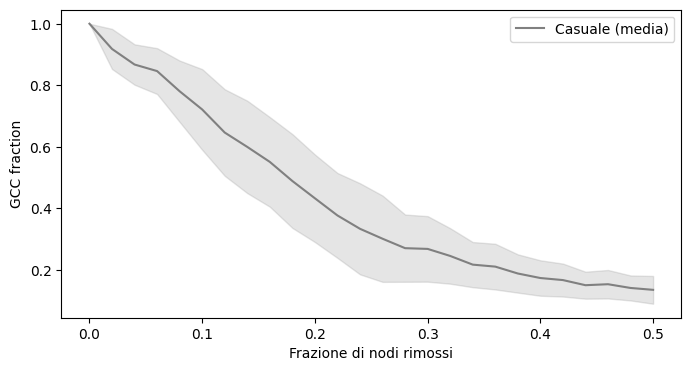
\includegraphics[width=0.8\linewidth]{Immagini//Capitoli//cap5/atk_random.png}
    \caption{Attacco di vulnerabilità casuale}
    \label{fig: Attacco di vulnerabilità casuale}
\end{figure}
\vspace{1em}

Il comportamento medio indica che il \textit{decadimento} è \textbf{graduale}, quasi \textbf{lineare}, serve rimuovere più del 20\% dei nodi per ridurre il GCC sotto il 50\%.

L'intervallo di confidenza resta relativamente ristretto ed evidenzia un comportamento stabile tra le simulazioni.

\subsection{Analisi dell'attacco per grado}
In figura \ref{fig: Confronto attacco di vulnerabilità per grado e per grado a cascata} è possibile visualizzare la \textit{GCC fraction} in relazione ai \textit{nodi rimossi} negli attacchi per grado, in un confronto tra un attacco mirato per grado e in un attacco a cascata per grado.

\vspace{1em}
\begin{figure}[ht!]
    \centering
    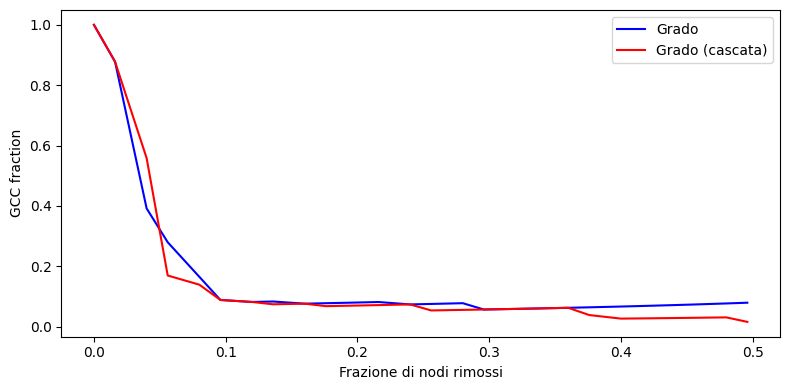
\includegraphics[width=0.8\linewidth]{Immagini//Capitoli//cap5/atk_degree_cfr.png}
    \caption{Confronto attacco di vulnerabilità per grado e per grado a cascata}
    \label{fig: Confronto attacco di vulnerabilità per grado e per grado a cascata}
\end{figure}
\vspace{1em}

Entrambe le curve \textbf{crollano} velocemente, la frazione del GCC scende sotto il 20\% già al 10\% dei nodi rimossi. \\
L'attacco a cascata leggermente più \textbf{aggressiva}. 

Dopo il 15\% di nodi rimossi, entrambe le curve si appiattiscono, indicando un collasso quasi totale della rete.

\subsection{Analisi dell'attacco per betweenness}
In figura \ref{fig: Confronto attacco di vulnerabilità per betweenness e per betweenness a cascata} è possibile visualizzare la \textit{GCC fraction} in relazione ai \textit{nodi rimossi} negli attacchi per betweenness, in un confronto tra un attacco mirato per betweenness e in un attacco a cascata per betweenness.

\vspace{1em}
\begin{figure}[h!]
    \centering
    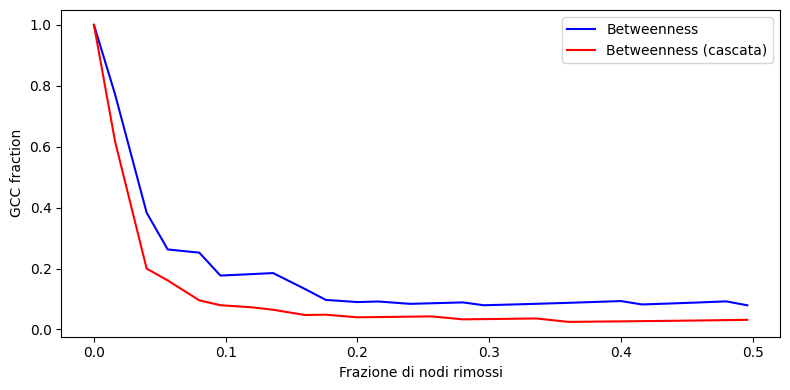
\includegraphics[width=0.8\linewidth]{Immagini//Capitoli//cap5/atk_btw_cfr.png}
    \caption{Confronto attacco di vulnerabilità per betweenness e per betweenness a cascata}
    \label{fig: Confronto attacco di vulnerabilità per betweenness e per betweenness a cascata}
\end{figure}
\vspace{1em}

Analogamente all'attacco precedente, entrambe le curve mostrano un \textbf{crollo} veloce, con una distruzione più repentina da parte dell'attacco \textit{a cascata}: dopo il 10\% dei nodi rimossi la rete è già quasi completamente frammentata.

La rete è dipendente da nodi con elevata betweenness, che fungono da intersezioni tra linee, e l’effetto cascata amplifica questa vulnerabilità: rimuovendo un nodo importante, altri ereditano la caratteristica e vengono rapidamente eliminati.

\subsection{Analisi comparativa degli attacchi}
In figura \ref{fig: Confronto attacchi di vulnerabilità} è possibile visualizzare la \textit{GCC fraction} in relazione ai \textit{nodi rimossi} in confronto a tutti gli attacchi esguiti.

\vspace{1em}
\begin{figure}[h!]
    \centering
    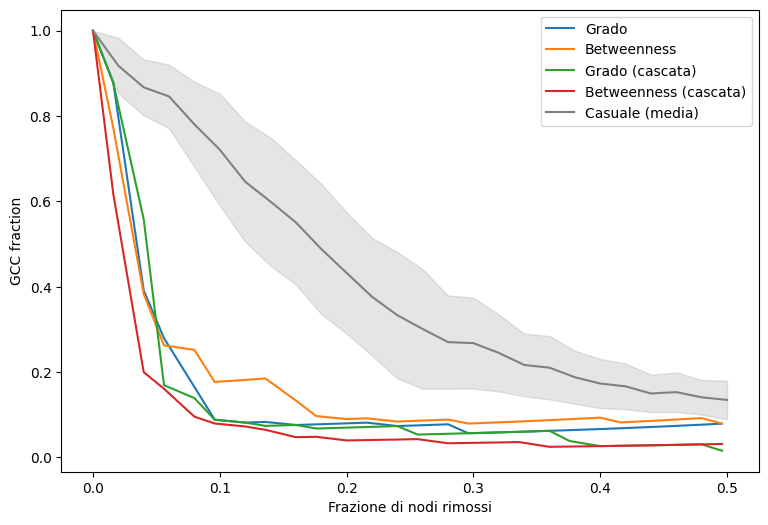
\includegraphics[width=0.8\linewidth]{Immagini//Capitoli//cap5/atk_cfr.png}
    \caption{Confronto attacchi di vulnerabilità}
    \label{fig: Confronto attacchi di vulnerabilità}
\end{figure}
\vspace{1em}

Operando il confronto, si conferma la decrescita \textbf{graduale} dell'attacco \textit{casuale}, rispetto alle altre tipologie di attacco che hanno una decrescita sensibilmente più \textbf{rapida}.

La rete metropolitana è quindi estremamente vulnerabile agli attacchi mirati su nodi con alto \textit{grado} o \textit{betweenness}, ma molto più robusta a f\textit{allimenti casuali}. Gli attacchi con effetto a cascata hanno l’impatto peggiore.

\vspace{1em}
\begin{figure}[h!]
    \centering
    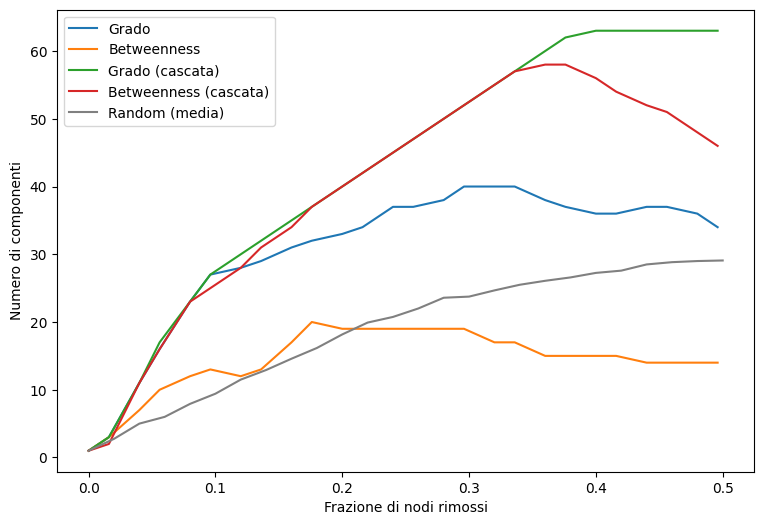
\includegraphics[width=0.8\linewidth]{Immagini//Capitoli//cap5/removed_cfr.png}
    \caption{Numero di componenti connesse in relazione alla rimozione di nodi}
    \label{fig: Numero di componenti connesse in relazione alla rimozione di nodi}
\end{figure}
\vspace{1em}

Un'altra analisi di confronto importante si può ritrovare in figura \ref{fig: Numero di componenti connesse in relazione alla rimozione di nodi}, in cui sono rappresentati il numero di componenti connessi nella rete che, partendo dall'unica iniziale, si degrada in più componenti connesse all'aumentare della frazione dei nodi rimossi.

Le curve degli attacchi a cascata crescono rapidamente e raggiungono oltre 60 componenti tra il 30\% e il 40\% di rimozione, la rete si frammenta \textbf{fortemente}.
La rimozione per grado mirata produce meno frammentazione, ma comunque notevole.

Una differenza rispetto alle analisi precedenti si ha nell'attacco per betweenness, che non produce un numero di componenti altrettato alto, tende quindi a isolare nodi mantenendo gruppi più compatti.

L'attacco casuale aumenta più lentamente e si stabilizza trai i 25 e i 30 componenti, coerentemente con la maggiore robustezza casuale.

Le strategie basate su grado o betweenness in modalità a cascata frammentano quindi rapidamente la rete, evidenziando che la connettività globale dipende da pochi nodi centrali critici. Gli attacchi per betweenness mirati creano meno frammentazione rispetto agli altri attacchi mirati, ma comunque distruggono la connettività principale come evidenziato precedentemente.

Le aspettative derivanti dalle analisi svolte nei capitoli precedenti sono state quindi \textbf{confermate} dai risultati degli attacchi svolti.